%!TEX TS-program = xelatex
%!TEX encoding = UTF-8 Unicode

\documentclass[onecolumn]{article}


%% LANGUAGE (english by default)
\def\mlanguage french % TODO: remove this and use a cli parameter
\usepackage{iflang}
\ifx\mlanguage\undefined
  \usepackage[frenchb, english]{babel}
  \selectlanguage{english}
\else
  \usepackage[english, frenchb]{babel}
  \selectlanguage{frenchb}
\fi
\newcommand{\ifr}[2]{\iflanguage{frenchb}{#1}{#2}}

%% PACKAGES %%
\usepackage[top=2cm,bottom=2cm,left=3cm,right=3cm]{geometry}
\usepackage[T1]{fontenc}
\usepackage[utf8]{inputenc}
\usepackage{url}
\usepackage{pdfpages}
\usepackage{graphicx}
\usepackage{lscape}
\usepackage{setspace}
\usepackage{titlesec}
\usepackage{sectsty}
\usepackage{placeins}
\usepackage{amsmath,amsfonts,amsthm}
\usepackage[hidelinks]{hyperref}
\usepackage[official]{eurosym}
\usepackage{fancyhdr}
\usepackage[sort&compress, authoryear]{natbib}
\usepackage{paralist} %% enumerate several elements on a single line like (i)
%% this is an example, (ii) this is a second example

%% TITLE PAGE
\title{
\normalfont \normalsize
\textsc{Université Pierre et Marie Curie} \\ [25pt]
\horrule{0.5pt} \\[0.4cm]
\huge Pré-rapport de stage\\
\horrule{2pt} \\[0.5cm]
}
\author{Pierre-Yves PÉNEAU}
\date{\normalsize\today}

%% HEADER / FOOTER
\pagestyle{plain}
\fancyhead{}
\fancyfoot{}
\fancyfoot[RO, LE] {\thepage}

\pagestyle{fancy}
\fancyhead{}
\fancyfoot{}

\fancyhead[CO,CE]{Pré-rapport de stage}
\fancyhead[LH]{Université Pierre et Marie Curie}
\fancyhead[RH]{Pierre-Yves Péneau}
\fancyfoot[C]{Draft version}
\fancyfoot[RO, LE] {\thepage}

%% COMMANDS
\newcommand{\todo}[1]{\textbf{\color{red}TODO: #1}}
\newcommand{\benumline}{\begin{inparaenum}[\itshape i\upshape)]}
\newcommand{\eenumline}{\end{inparaenum}}
\setlength\parindent{0pt}
\titleformat{\chapter}[hang]{\bf\huge}{\thechapter}{2pc}{}
\newcommand{\horrule}[1]{\rule{\linewidth}{#1}}
\renewcommand{\headrulewidth}{0.4pt}
\renewcommand{\footrulewidth}{0.4pt}
\bibpunct{[}{]}{,}{n}{,}{,}
%% 1/ The symbol for the opening bracket.
%% 2/ The symbol for the closing bracket.

%% 3/ The symbol that appears between multiple citations.
%%      This argument takes a letter:
%%       n - numerical style.
%%       s - numerical superscript style.
%%       any other letter - author-year style.

%% 4/ The punctuation to appear between the author and the year (in
%% parenthetical case only).

%% 5/ The punctuation used between years, in multiple citations when there is a
%% common author. e.g., (Chomsky 1956, 1957). If you want an extra space, then
%% you need {,~}.

%% Misc
\graphicspath{{include/img/},{include/pdf/}}
\DeclareGraphicsExtensions{.jpeg,.jpg,.png}

\begin{document}

  \maketitle
  \tableofcontents
  \onehalfspacing
 
  \ifr{ %% FRENCH PART HERE
    \chapter{Introduction}

  Au milieu des années 2000, les fabricants de processeurs ont atteint une
  limite technique.  Au-delà de 100 Watts par boitier, il est difficile de
  refroidir les circuits à l'aide de simples ventilateurs. Les technologies
  comme le \textit{water cooling}~\citep{googleXXXXdatacenters} sont coûteuses
  et énergivores.  Pour continuer l'augmentation de puissance des processeurs en
  profitant de la loi de Moore, ils ont dû cesser de complexifier l'architecture
  des c\oe urs et d'augmenter leur fréquence de fonctionnement. Au contraire,
  ils ont simplifié les c\oe urs pour en mettre plusieurs par processeur.  De
  nos jours, les architectures à 8 c\oe urs sont courantes, celles à une
  cinquantaine de c\oe urs sont disponibles, et d'autres comportant plusieurs
  centaines, voire milliers, sont à prévoir.  L'augmentation du nombre de c\oe
  urs par processeur permet l'augmentation du nombre d'instructions exécutées
  par cycle.  Cela impose une augmentation de la quantité de mémoire nécessaire
  et du débit des accès~\citep{hp2012z820, puget2013z9pe}. Les systèmes
  d'exploitation doivent s'adapter pour gérer efficacement ces nouvelles
  ressources.\\

  Dans ce stage, l'architecture matérielle considérée est l'architecture
  TSAR~\citep{greiner2009tsar}\nomenclature{TSAR}{Tera-Scale Architecture}
  développée au LIP6\nomenclature{LIP6}{Laboratoire d'Informatique de Paris
    6}. TSAR est une architecture NUMA\nomenclature{NUMA}{Non-Uniform Memory
    Access} à mémoire partagée cohérente, composée de 1024 c\oe urs 32 bits et
  1To de mémoire physique (40 bits).  Les c\oe urs sont répartis en clusters
  contenant chacun 4 c\oe urs et gérant un segment de 4Go de mémoire
  physique. Le choix de c\oe urs 32 bits, et non 64 bits, est assumé. C'est,
  selon les architectes, le meilleur compromis en énergie dissipée par
  instruction, et cela permet un meilleur usage des caches car les pointeurs
  sont plus petits.  Un système d'exploitation nommé
  ALMOS~\citep{almaless2011almos}\nomenclature{ALMOS}{Advanced Locality
    Management Operating System} a été spécialement développé pour TSAR. Ce
  système est basé sur un noyau monolithique, tout comme Linux ou
  *BSD\nomenclature{BSD}{Berkeley Software Distribution}. ALMOS signifie
  \textit{Advanced Locality Management Operating System}. En effet, son but
  premier est le placement efficace des données dans les segments mémoires, et
  des threads accédant à ces données sur les c\oe urs.\\

  L'architecture TSAR utilisée lors du développement d'ALMOS n'était pas
  finalisée. Elle ne proposait que 4Go de mémoire physique (32 bits). Elle gère
  désormais 1To (40 bits). Le but de ce stage est de faire évoluer ALMOS pour
  permettre la gestion de ce tera octet.\\

  Nous faisons face à plusieurs problèmes. Le premier est que les c\oe urs 32
  bits sont limités à 4Go d'espace adressable virtuel. Le noyau doit gérer un
  espace mémoire physique supérieur à l'espace virtuel des processeurs. Pour
  résoudre ce problème, nous verrons que nous allons devoir répartir et souvent
  répliquer toutes les structures du noyau dans chaque cluster. ALMOS, dans sa
  version 32 bits, a déjà une organisation clusterisée pour gérer le
  co-placement des threads et des données, mais cela n'interdit pas d'accéder
  facilement à toute la mémoire; c'est désormais difficile. Le deuxième problème
  est donc de revoir la répartition ou réplication des structures du noyau et
  leur mode d'accès. ALMOS va ainsi évoluer vers une structure semblable par
  certains aspects au multi-noyau~\citep{baumann2009multikernel}. Ainsi, le
  troisième problème est une conséquence du deuxième. Si certaines structures
  sont répliquées, il faut que le système en garantisse la cohérence pour offrir
  à l'utilisateur l'illusion d'un noyau monolithique. \\

  Pour ce stage, nous allons nous concentrer sur les structures partagées par
  les threads d'un processus, telles que les descripteurs de fichiers ou les
  zones mémoires partagées. \\

  Ce document est organisé de la manière suivante: en section~\ref{sec:memory}
  nous nous intéresserons à la gestion de grande quantité de mémoire sur des
  architectures 32 bits. En section~\ref{sec:scalability} nous présenterons les
  différents travaux de recherche adressant la problématique du passage à
  l'échelle des systèmes d'exploitation.  La section~\ref{sec:consistency} est
  relative aux problèmes de cohérence mémoire pour les structures de données des
  noyaux large échelle. La présentation du contexte de travail sera faite en
  section~\ref{sec:context}. Enfin nous concluerons en
  section~\ref{sec:conclusion}.\newline

    \section{État de l’art}

  La problématique du passage à l’échelle des noyaux n’est pas nouvelle. En
  effet, dès les années 90, ~\citeauthor{unrau1995hierarchical} posent la
  question et apportent des réponses avec le noyau Hurricane. D’autres ont
  également essayé avec le micro-noyau L4. Mais ce fut finalement Linux qui
  s’imposa comme le modèle de référence, et les travaux focalisèrent alors sur
  ce dernier.

  Mais, aux alentours des années 2004-2005, un changement radical a été opéré de
  la part des construc- teurs tels qu’Intel ou AMD. Plutôt que de continuer à
  augmenter la fréquence des processeurs, ce qui devenait contre productif vu la
  quantité d’énergie nécessaire, ils ont préféré augmenter le nombre de coeurs
  et le nombre de processeurs sur les puces. C’est ainsi que l’ère du
  parallélisme massif commenca~\citep{patterson2011parallel}, et que la
  problématique du passage à l’échelle du noyau Linux fût soulevée.

  En plus de cette problématique, il nous paraît important de mettre l’accent
  sur un phénomène rare en informatique, et qui est au c\oe ur de notre
  étude. En effet, le mélange de l’architecture TSAR et du noyau ALMOS fait que
  nous nous retrouvons ici à devoir gérer un espace d’adressage physique plus
  grand que l’espace d’adressage virtuel offert par le noyau.

  Enfin, le passage d’ALMOS au mode multi-noyau nous permettra de voir comment
  les différentes solutions existantes maintiennent cohérentes des structures de
  données vitales au fonctionnement du noyau


  \subsection{Passage à l’échelle des noyaux}
  \label{sec:scalability}

    \subsubsection{Scalabilité du noyau Linux}

      Il apparait évident dans un premier temps de vouloir adapter le noyau
      Linux à des architectures massivement multi-coeurs. En effet, changer de
      noyau, alors que ce dernier s’est imposé partout, est un pari très risqué,
      et très difficile. Pour imposer un nouveau noyau, il faudrait que ce
      dernier soit en adéquation parfaite avec l’API proposée par Linux, et ce
      pour que le fonctionnement des applications actuelles, et le développement
      de futures application, soit le plus transparent possible pour
      l’utilisateur ou le développeur. À cet effet, ~\citet{boyd2010analysis}
      ont étudié la scalabilité de Linux sur une machine
      48 coeurs, et utilisant le benchmark MOSBENCH. Ils ont pu tirer plusieurs
      conclusion de cet études.  Premièrement, il existe trois type de problème
      liés au passage à l’échelle :
      \begin{itemize}
        \item l’implémentation du noyau
        \item l’implémentation de l’application utilisateur
        \item la manière dont l’application utilise les services noyau
      \end{itemize}
      Grâce à cela, ils sont parvenus à résoudre les problèmes liés aux
      applications relatives à MOSBENCH, et ce en utilisant des techniques
      basique de programmation parallèle. De plus, la grande majorité de leurs
      contributions sur le noyau ne sont que de petits changements, et très
      localisés. À l’exception faite des \textit{sloppy counters}, aucun concept
      clé de Linux n'a été touché

      Ainsi, ils sont parvenus à identifier les problèmes du noyau, comme par
      exemple la gestion du cache des dentry, les goulots formés par les sytèmes
      de fichiers montés, etc\ldots, et à les résoudres pour obtenir des
      performances acceptables.

      Néanmoins, nous pouvons aujourd’hui adresser trois critiques à ceus
      travaux :
      \begin{itemize}
        \item le noyau utilisé est ancien (2.6.35-rc5, 12 Juillet 2010). Les
          mécanismes de prémption venaient d’être ajoutés et n’étaient pas aussi
          performants que maintenant.
        \item la machine considérée est composée de seulement 48 coeurs, ce qui
          est peu par rapport à la puissance des machines d’aujourd’hui
        \item leur propre conclusion indique qu’il ne faut pas changer le design
          des sytèmes d’exploitation `` pour l’instant''
      \end{itemize}
      Nous pensons qu’à présent, il est nécessaire de revoir cette organisation.

      
    \subsubsection{Popcorn Linux}

      Le projet Popcorn Linux~\citep{barbalacepopcorn} part du même constat
      évoqué précédement, mais en essayant tout de même de conserver le noyau
      Linux comme base de travail. Avec un noyau plus actuel que précédement
      (3.2), ils ont en partie adopté les principes du multi-noyau mais en ont
      rejetés certain.

      Popcorn Linux permet de lancer plusieurs noyau Linux en même temps sur la
      même machine, Le matériel est attribué de manière logicielle entre les :
      différentes instances du noyau, et ces dernières communiquent uniquement
      par passage de messages. Afin de garantir à l’utilisateur l’illusion d’un
      seul système en exécution, ils ont utilisé les mécanismes de
      \textit{namespace} offert par Linux pour construire ce qu’ils appellent ``
      l’image disque unique'' (\textit{Single System Image}).

      Le partitionnement des ressources est fait selon la configuration donnée
      au boot du noyau. Le premier noyau qui est lancé, appelé `` noyau
      maître'', lance un processus de reconnaissance du matériel. Ensuite, on
      précise au noyau via des paramètres au boot, les ressources dont il peut
      disposer, en fonction de celle trouvées par le noyau maître. Une fois les
      noyaux lancés, ils ne partagent aucune données, exception faite de la
      table contenant les adresse d’écriture des buffers des autres noyaux,
      utilisés pour le passage de messages. Ces buffers sont de types `` MWSR'',
      ou \textit{Multi Writer Single Reader}, et utilisent un système de ticket
      pour les écritures. Les lectures utilisent un mélange de deux
      techniques:\benumline \item le lecteur vient consulter de manière
      régulière le contenu de son buffer (\textit{polling}) \item il ira lire le
      buffer sur réception d’une IPI (\textit{Inter-Processor Interruption}) du
      coeur ayant initié l’écriture\eenumline.

      Ces communications permettent de donner l’illusion qu’il n’y a qu’un seul
      noyau en cours d’exécution, mais aussi de pouvoir migrer des tâches entre
      les différentes instances de noyaux de manière transparente.

      
    \subsubsection{Hurricane}

      Parmi les premiers travaux sur la scalabilité des systèmes d’exploitation
      se trouve la thèse d’Unrau Celui-ci a formulé trois grands principes pour
      une conception scalable d’un système d’exploitation qui sont :
      \benumline \item préserver le parallélisme \item borner le surcoût des
      services et \item préserver la
      localité\eenumline. \citet{unrau1995hierarchical} ont proposé le système
      d’exploitation Hurricane à base de micro-noyau avec une approche de
      conception nommée Hierarchical Clustering.

      Selon cette approche, le système d’exploitation est vu en tant qu’une
      collection de clusters. Un cluster est un système d’exploitation complet
      à base de micro-noyau prenant en charge un faible nombre de
      processeurs. Il existe donc autant d’instances du système d’exploitation
      que de clusters. Les serveurs systèmes (en mode utilisateur) de chaque
      cluster coopèrent entre- eux pour donner aux applications une vision
      globale d’un seul système d’exploitation. Étant donné que chaque cluster
      propose l’ensemble des services système via des serveurs dédiés,
      l’existence de plusieurs clusters constitue une réplication des mêmes
      services et augmente la disponibilité du système. La dimension (en nombre
      de processeurs) d’un cluster est un compromis entre le coût des accès
      intra-cluster et inter-clusters.
      %%
      %% La figure~\ref{fig:hurricane} illustre l’organisation de plusieurs
      %% clusters pour constituer un système distribué fortement couplé.

      %% \begin{figure}[h]
      %%   \centering
      %%   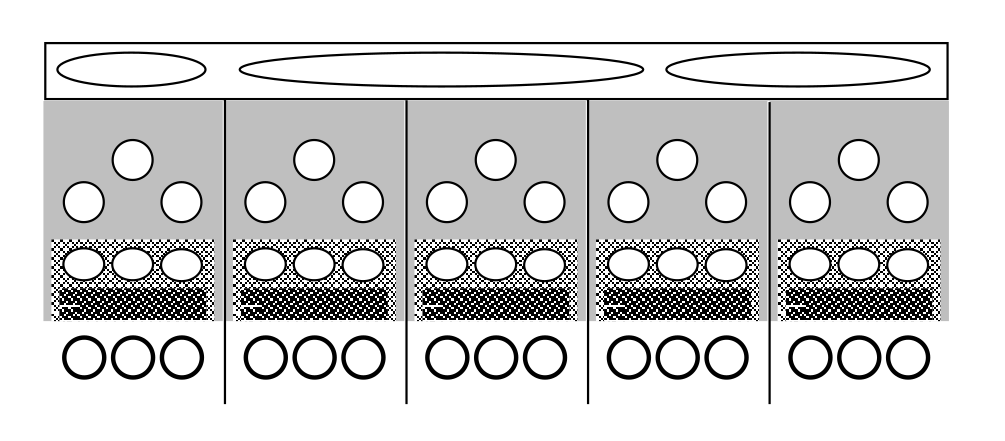
\includegraphics[scale=0.3]{hurricane}
      %%   \caption{Un système multi-cluster}
      %%   \label{fig:hurricane}
      %% \end{figure}
      %%
      Dans Hurricane, chaque cluster dispose de son propre ordonnanceur qui
      assure localement l’équilibrage de charge et l'ordonnancement des
      processus, tandis que l’équilibrage de charge inter-clusters est assuré
      par un ordonnanceur global. Les communications dans Hurricane peuvent être
      réalisées par l’envoi de messages ou par l’utilisation de Protected
      Procedure Calls (PPC).

      Un envoi de message est réalisé par l’interruption du cluster cible
      pour\benumline \item l’allocation d’un tampon mémoire pour réceptionner le
      message \item copier le message et les informations de contrôle depuis le
      processus émetteur du cluster source et \item attacher le tampon à la file
      d’attente du processus destinataire du message\eenumline.

      Quant un client demande un service, il change son espace d’adresse pour
      celui du serveur et invoque un thread de traitement associé à sa requête
      avant de retrouver son espace d’adressage initial.


    \subsubsection{Corey}

      Avant leurs travaux sur Linux,~\citet{boyd2008corey}. ont proposé le
      système d’exploitation Corey. Dans ce dernier, la gestion du partage des
      ressources est laissé aux applications utilisateurs.

      En donnant le contrôle aux programmeurs des applications utilisateur,
      Corey permet en effet de per- sonnaliser le comportement du noyau selon
      les besoins et les spécificités d’une application. Les inconvénients
      majeurs de cette approche sont: \benumline \item lier fortement l’application au
      système qui l’exécute, ce qui élimine complètement ou partiellement la
      portabilité des applications et complique sérieusement la réutilisation du
      code existant \item augmenter la complexité de programmation et
      nécessiter d’avantage d’efforts de la part des programmeurs d’applications
      (gestion explicite des régions virtuelles, placement et partage des
      structures de données noyau, etc.) et \item  générer des conflits entre
      les choix propres de chaque application dans le contexte de l’exécution
      dynamique de plusieurs applications simultanées\eenumline.


    \subsubsection{Barrelfish}
      
      L’ETH Zurich, en collaboration avec Microsoft Research, a engagé des
      travaux de recherches dans le domaines des architectures du futures en
      2008. Leur équipes sont arrivées à établir un nouveau modèle d’élaboration
      des systèmes d’exploitation : le
      multi-noyau~\citep{schupbach2008embracing}. Ce paradigme part de plusieurs
      postulats\benumline \item les architectures du futures seront très
      hétérogènes \item les noyaux actuels ne profite pas de l’hétérogénéité
      offertes par le matériel et au contraire essaye de la masquer un maximum
      \item les machines sont construites comme des systèmes distribués, pourquoi
        ne pas appliquer le même modèle aux systèmes d’exploitation\eenumline.

      \begin{figure}
        \centering
        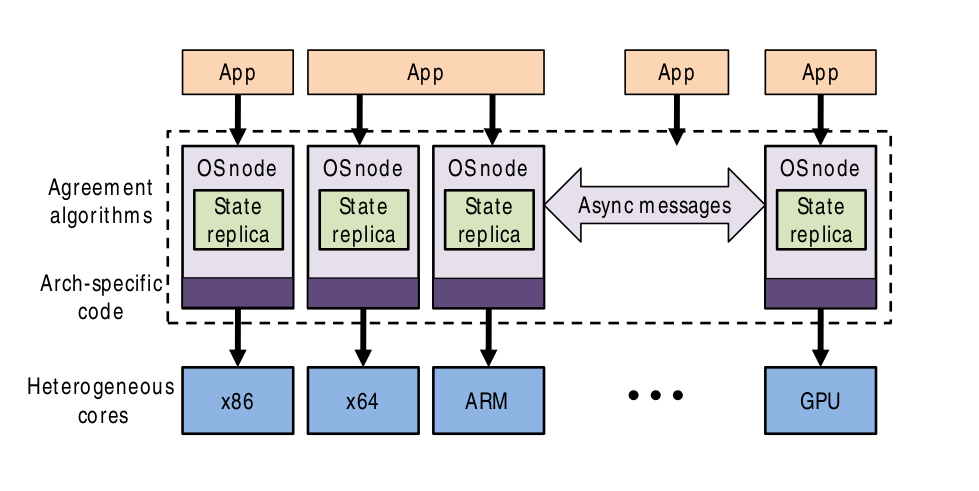
\includegraphics[scale=0.3]{barrelfish}
        \caption{L'architecture multi-noyau. Source:
          \citeauthor{schupbach2008embracing}}
        \label{fig:barrelfish}
      \end{figure}
        
      Selon l’approche multi-noyau (voir figure~\ref{fig:barrelfish}),
      l'environnement d’exécution des applications est une collection de n\oe
      uds où chaque n\oe ud est constitué d’un c\oe ur exécutant un OS à base
      d’un micro-noyau. Les communications entre les différentes OS se font par
      passage de messages : Barrelfish utilise une variante des Remote Procedure
      Calls au niveau utilisateur (URPC). chaque OS dispose d’un serveur système
      en mode utilisateur appelé Monitor. L’ensemble des moniteurs coordonnent
      collectivement l’accès à l’état global du système et maintient la
      cohérence des structures de données répliquées par c\oe ur (les tables
      d’allocation mémoire et les mappings des espaces d’adressages
      virtuels). La notion d’un processus dans Barrelfish est différente de
      celle d’un processus dans un noyau monolithique. Un processus est
      représenté sous formes d’un ensemble de Dispatchers avec un Dispatcher par
      c\oe ur où le processus peut être exécuté. Sur un c\oe ur, les Dispatchers
      sont ordonnancés par un ordonnanceur, au niveau du micro-noyau de ce c\oe
      ur, appelé CPU Driver. Ce dernier communique avec les Dispatchers (en mode
      utilisateur) à travers des up-calls.\newline
      

    \subsubsection{Influences}

      Bien que ces travaux n'apportent pas de réponses claires et définitives à
      notre problématique, il nous permettent de mieux comprendre les choix qui
      ont été fait dans le noyau ALMOS. Premièrement, les travaux sur Barrelfish
      ont apporté un nouveau modèle architectural pour la conception d'un
      noyau. Ce modèle semble cohérent et répond aux beoins des futures
      architectures. C'est donc le modèle qui a été retenu par
      ALMOS\footnote{Nous verrons plus en détail en section~\ref{sec:almos} le
        choix du multi-noyau.}. Néanmoins, Barrelfish ne respecte pas du tout
      les standards POSIX. C'est un choix très fort qui a été pour ce projet, et
      qui nous apparaît comme infondé.

      Les travaux sur Popcorn Linux, basé lui aussi sur le modèle du
      multi-noyau, ont permis de montrer que le noyau Linux, qui se veut être
      \textit{POSIX compliant}, peut être adapté à des architectures massivement
      parallèles, tout en respectant les normes. Le projet ALMOS, tout comme
      Popcorn Linux, a fait le choix d'avoir un système respectant au maximum
      les standards de conception des noyuax déja existants.

      Pourtant, ces recherches ne répondent pas à un des problèmes majeurs de
      l'architecture TSAR. En partant du principe que les processeurs
      d'aujourd'hui manipulent des informations sur 64 bits, les problèmes de
      gestion d'une grande quantité de mémoire ont été effacés. Nous allons tout
      de même présenter en section~\ref{sec:memory} quelques solutions
      permettant de contourner ce problème, mais toujours de manière incomplète.
    
     

  \subsection{Gestion des espaces d'adressage}
  \label{sec:memory}    

    \subsubsection{Les processeurs}

      MIPS registers\\
      PAE Intel


    \subsubsection{Linux, OpenBSD et NetBSD}
  
      Un des problèmes des espaces physiques de grande taille est la tables des
      descripteurs de pages physiques\footnote{L’utilisation du mot “table” est
        un abus de langage : dans les systèmes modernes, c’est en réalité une
        liste doublement chainée}. En effet, lors de l’initialisation du
      système, ce dernier crée tous les descripteurs de pages nécessaires pour
      décrire toute la mémoire physique de la machine~\citep{cranor1999uvm,
        gorman2004understanding}. Lorsque l’on dispose d’une grosse quantité de
      mémoire, la taille de cette table est énorme. A titre d’exemple, ALMOS à
      besoin de 14Go pour décrire les 1To de mémoire offerts par TSAR. Cette
      valeur, bien qu’élevée, est largement supérieure dans les noyaux Linux,
      OpenBSD et NetBSD, car les structures représentant les pages dans ces
      noyaux sont plus volumineuses en mémoire que celle d’ALMOS.

      Du fait de la taille énorme de ces descripeurs, le problème apparaît
      rapidement : comment stocker 14Go de données lorsque l’on a que 1Go
      d’espace virtuel ?  La réponse est simple : on ne peut pas.  Ainsi, les
      noyaux cités précédemment ne peuvent pas gérer plus de 4Go de mémoire dans
      leur versions 32 bits.


    \subsubsection{Le cas FreeBSD}

      Selon la documentation, il apparaît que le noyau de FreeBSD soit le seul
      capable de gérer une telle situation. Les développeurs indiquent que le
      noyau peut gérer jusqu’à 8To de mémoire, le tout en utilisant des tailles
      d’adresses de 32 bits~\citep{kernelfreebsd, mckusick1996design}.

      \todo{Je suis en train de voir ca sur une mailing-liste. Apparement il
        manquerait simplement un support MIPS pour certaines choses mais sinon
        ça devrait marcher (en tout cas pour la gestion d'1To de mémoire).}

      
  \subsection{Partage et maintient de cohérence de structures noyaux}
  \label{sec:consistency}
  
    %% \subsubsection{Hare}

    %% \subsubsection{Barrelfish}

    %%   passage de message

    %% \subsubsection{DragonFly BSD}

    %%   multi-noyau, passage de message, HAMMER

    \chapter{Contexte de travail}
\label{sec:context}

  Pour répondre à ces enjeux de passage à l'échelle et de consommation
  énergétique, l'équipe ALSOC du LIP6 participe à deux projets d'envergures:
  TSAR~\cite{tsar2008} et SHARP~\cite{sharp2012}. Le premier a pour but de
  fournir une architecture matérielle passant à l'échelle de plusieurs centaines
  de coeurs, tandis que l'autre se veut être capable de fournir un système
  d'exploitation pour gérer efficacement cette nouvelle architecture.

  Notre travail portera sur le multi-noyau ALMOS, et plus particulièrement sur
  la migration de tâches entre différentes instances du noyau. Nous allons dans
  un premier temps présenter l'architecture matérielle TSAR. L'étude de cette
  dernière est essentielle pour bien comprendre les enjeux d'ALMOS. Ensuite nous
  présenterons le noyau ALMOS, et notamment son cycle de vie, et enfin nous
  concluerons sur le travail que nous allons effectuer dans le cadre de ce
  stage.
  

  \section{L'architecture TSAR}
  \label{sec:tsar}

    TSAR est l'architecture d’un processeur multi-c\oe urs cc-NUMA homogène
    pouvant intégrer jusqu’à 4096 c\oe urs~\cite{greiner2009tsar}. Cette
    architecture est le résultat d’un projet de recherche européen
    MEDEA+~\cite{tsar2008} dont les principaux partenaires industriels sont
    BULL, Philips et THALES, et dont les partenaires académiques sont le LIP6 et
    le CEA-Leti. La figure \ref{fig:tsar} illustre un aperçu global de
    l'architecture TSAR. Il s'agit d'un ensemble de clusters interconnectés par
    un NoC (\textit{Network-On-Chip}) DSPIN (\textit{Distributed, Scalable,
      Predictable, Integrated Network}). Chaque c\oe ur dispose de ses propres
    caches L1 indexés en adresses physiques (données et instructions séparés) et
    d'une MMU (Memory Management Unit). La cohérence des caches de premier
    niveau de tous les c\oe urs ainsi que des TLBs est assurée par un protocole
    matériel nommé DHCCP (\textit{Distributed Hybrid Cache Coherence
      Protocol}). Une description complète de cette architecture est disponible
    sur le site du projet TSAR~\cite{tsar2008web}.

    \begin{figure}[ht]
      \centering 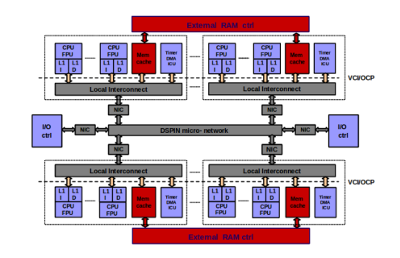
\includegraphics[scale=0.2]{include/img/tsar.png}
      \caption{Schéma global de l'architecture TSAR~\citep{greiner2009tsar}.}
      \label{fig:tsar}
    \end{figure}

    Dans la suite de ce document, on considére la version TSAR-Leti comme étant
    l'architecture de base. Celle-ci contient 4096 processeurs réparti en 256
    clusters de 4 processeurs chacun. La mémoire vive est de 1To, et chaque
    cluster gère un segment de 4Go. Lors de la mise sous tension, c'est le
    cluster 0 qui est chargé d'initialiser tout le système.

  \section{Le noyau ALMOS}
  \label{sec:almos}

    Le noyau ALMOS~\cite{almaless2011almos} est un noyau monolithique
    expérimental developpé au LIP6 par l'équipe ALSOC depuis 2011. Sujet de
    thèse de Ghassan Almaless, le développement est maintenant à la charge de
    Mohamed Karaoui (système de fichiers) et Clément Devigne (exécution de
    machines virtuelles). Le but d'ALMOS est de répondre à la problématique
    évoquée de la localité des accès mémoires dans les machines cc-NUMA. Une des
    particularités dans les choix architecturaux d'ALMOS est d'avoir choisi de
    développer un noyau monolithique. Il respecte la norme
    POSIX~\cite{posix2013} et implémente différentes libraires:
    \texttt{libpthread, mpi, openMP}\ldots Le but premier d'ALMOS est de
    garantir un passage à l'échelle et une conservation de la localité des accès
    mémoires. Pour cela, le noyau intègre trois nouveaux mécanismes:
    \benumline \item les clusters managers \item les réplica-noyau \item une
    nouvelle stratégie d'allocation mémoire (\textit{Auto-Next-Touch})
    \eenumline.

    
    \subsection{Les cluster-manager}

      L'organisation distribuée du noyau ALMOS s’appuie sur les objets nommés
      \textit{cluster-manager}. L’objectif est d’une part, de décentraliser la
      gestion des ressources et d’autre part, d’assurer une localité d’accès
      mémoire lors de cette gestion. Un cluster-manager est un objet responsable
      de la gestion des ressources physiques (essentiellement c\oe urs et
      mémoire physique) d’un nœud cc-NUMA. Il existe autant de cluster-manager
      qu’il y a de clusters. Chacun d'eux est placé localement dans la mémoire
      physique de son n\oe ud. Comme l'illustre la figure
      ~\ref{fig:cluster_manager}, ils contiennent, entre autre, un
      \textit{memory-manager} et un ou plusieurs \textit{core-manager}.  Ce
      dernier est un objet responsable de la gestion d’un c\oe ur et plus
      précisément de l'ordonnancement des tâches affectées à ce c\oe ur ainsi
      que de la gestion des événements reçus par ce c\oe urs. L'ordonnancement
      est assuré par un serveur d'ordonnancement appelé
      \textit{scheduler-server}, tandis que la gestion des événements est
      assurée par \textit{l'events-manager}. Le \textit{memory manager} est
      quant à lui responsable de l'allocation et la gestion de la mémoire sur le
      cluster.

      \begin{figure}[ht]
        \centering 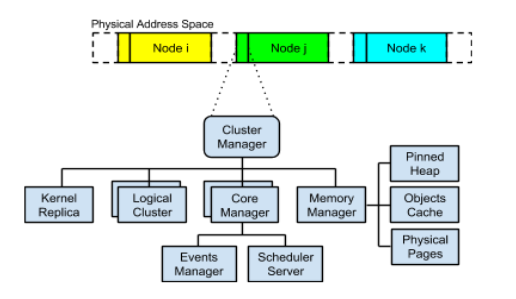
\includegraphics[scale=0.22]{include/img/cluster_manager}
        \caption{Un \textit{cluster manager} est un gestionnaire de ressources
          d'un n\oe ud cc-NUMA. Il est physiquement placé dans le banc mémoire
          du n\oe ud correspondant~\citep{almaless2014universite}.}
        \label{fig:cluster_manager}
      \end{figure}

      
    \subsection{Les réplica noyau}

      Comme nous l'avons vu précédemment, l'architecture TSAR offre au système
      d'exploitation la notion de cluster. Ceux-ci sont composés de quatre
      processeurs connectés entre eux sur un interonnect local, lui-même relié à
      différents périphériques (TTy, ICU, NIC, etc\ldots).
      
      La norme POSIX impose\footnote{\todo{C'est vraiment la norme qui impose ća
          ou on peut tout simplement pas faire autrement ?}} que dans l'espace
      d'adressage des processus, il y ait un mapping sur certaines pages du
      noyau. Or, si le code et les données du noyau sont situés à un seul et
      unique endroit en mémoire physique, et que chaque processus mappe ces
      pages dans son espace virtuel, alors on paiera le coût de l'architecture
      NUMA à chaque appel système, puisque l'on devra accéder à des pages
      distantes.

      Afin de résoudre ce problème, la notion de réplica noyau a été introduite
      au sein des \textit{clusters-manager}. Un réplica noyau consiste à
      dupliquer le code du noyau et les données partagées dans les premières
      pages physiques de chaque cluster. Ces pages sont en lecture seule pour
      garantir la cohérence et la sécurité. Lors de la création d'un processus,
      les pages qui représentent le noyau correspondent aux pages physiques du
      cluster sur lequel le processus vient d'être créé.


  \section{Évolution du projet}

    \subsection{Limitations de la version initiale}
    
      Développé initialement pour une architecture 32 bits, le noyau ne peut pas
      supporter plus de 4Go de mémoire vive. L'objectif visé n'était pas de
      supporter le téra-octet de mémoire de TSAR, mais de supporter le passage à
      l'échelle de plusieurs centaines de coeurs. Ainsi, un des premiers
      problème d'ALMOS est le mapping de l'espace virtuel, qui se révèle être
      très simple. En effet, lors de la phase de boot, ce dernier va chercher à
      mapper le maximum de la mémoire physique du cluster de boot dans son
      espace virtuel\footnote{Contraitement aux noyaux ``classiques'', ALMOS
        s'accordge 2 giga-octet d'espace virtuel au lieu de 1.}. Donc, si ce
      cluster possède (au moins) 2Go de mémoire physique, l'ensemble du noyau
      est mappé dans ce seul cluster. De plus, cela ne laisse que 2Go de mémoire
      virtuelle pour les applications utilisateur.

      
    \subsection{Contributions de Francois \citeauthor{guerret2014exploitation}}
      
      La gestion d'une telle quantité de mémoire fut le sujet de stage de
      Francois~\citet{guerret2014exploitation} en 2014. Ce dernier proposa
      différents changements pour ALMOS : \benumline \item réduire l'espace
      virtuel noyau à 1Go \item répartir cet espace virtuel entre les
      clusters \item sortir de l'espace virtuel les structures de données du
      noyau de taille importante \eenumline. Ces changements sont représentés
      par la figure~\ref{fig:almos-guerret}.

      \begin{paragraph}{Répartition de l'espace d'adressage noyau:}
        Celle-ci est calculée en fonction du nombre de clusters de
        l'architecture ($\frac{\text{Taille virtuelle}}{\text{Nb
            clusters}}$). Pour une architecture TSAR-Leti 40 bits, on dispose de
        256 clusters, on a donc $\frac{1000}{256}\approx4$Mo d'espace virtuel
        noyau par cluster.
      \end{paragraph}

      \begin{figure}[ht]
        \centering 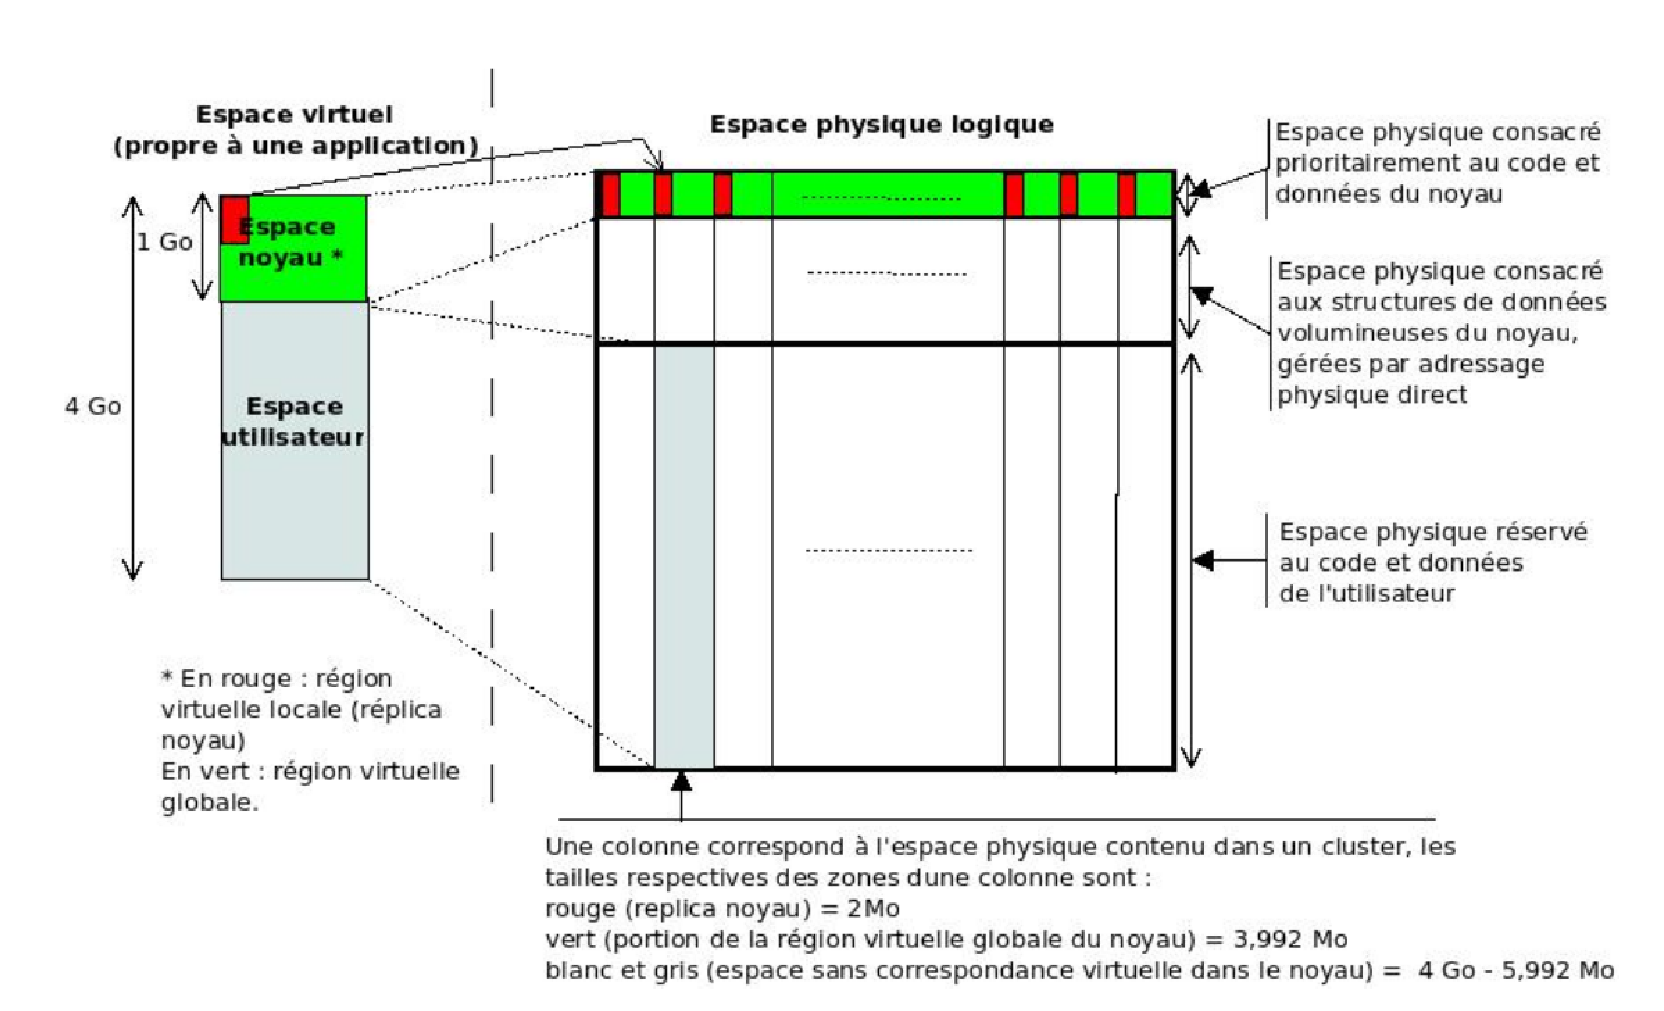
\includegraphics[scale=0.33]{include/img/almos-guerret}
        \caption{Répartition de l'espace virtuel du noyau tel que proposé par
          Franćois \citet{guerret2014exploitation}.}
        \label{fig:almos-guerret}
      \end{figure}

      \begin{paragraph}{Gestion en adressage physiques de structures de données:}
        Avec 4Mo d'espace virtuel noyau par clusters, certaines structures de
        données ne pouvait plus être contenues dans un si petit espace, comme
        par exemple la table des pages. Celle-ci, une fois pleine\footnote{Ce
          cas n'arrive jamais, mais il est néanmoins mathématiquement possible},
        peut atteindre une taille maximale de 8Mo. De plus, chaque processus
        dipose de sa propre table des pages. Il est techniquement impossible de
        stocker 8Mo dans cet espace virtuel, Francois a donc choisi de sortir
        cette structure de l'espace virtuel.

        La seconde structure de données problématique est la table des
        descripteurs de pages physiques. Les noyaux actuels ont fait le choix de
        décrire toutes les pages physiques qu'offre la mémoire. Ainsi, pour
        décrire le tera-octet de mémoire offert par TSAR, il est nécessaire
        d'utiliser 14Go de mémoire, soit 56Mo par cluster. Une fois de plus, il
        est impossible de stocker cette structure dans l'espace virtuel
        noyau. Celle-ci a donc été sortie et est gérée en adressage physique.
      \end{paragraph}

      \begin{paragraph}{Résultats:}
        Ce travail n'a malheureusement pas donné lieu à une solution
        fonctionnelle. La gestion par des adresses physiques des ces deux
        structures s'est avérée être très compliquée et nécessitait de recoder
        une partie conséquente du noyau. Le principal inconvénient de ce choix
        est le parcours de listes: il est nécessaire de vérifier que chaque
        élément n'est pas une structure gérée physiquement avant de pouvoir
        l'accéder. Cela allourdi considérablement l'opération, cette solution
        fût donc abandonnée. Néanmoins, elle a ouvert la voie à la version
        suivante d'ALMOS.
      \end{paragraph}

      
  \section{Passage au mode multi-noyau}
  \label{sec:multi-noyau}

    La version actuelle d'ALMOS proposée par Mohamed Karaoui et Franck Wajsbürt
    supprime totalement l'espace virtuel du noyau. Ce dernier fonctionne
    entièrement en adressage physique et passe en mode multi-noyau, avec une
    instance de noyau dans chaque cluster. Ces changements permettent de gérer
    toute la mémoire physique de la plateforme TSAR, puisque \benumline \item
    chaque cluster dispose de 4Go de mémoire physique \item on a un noyau par
    cluster \item le noyau peut gérer 4Go de mémoire\eenumline. Ce changement
    permet également de laisser 4Go de mémoire virtuelle\footnote{Modulo une
      page de petite taille (4Ko) pour faire le passage entre le mode
      utilisateur et le mode noyau} à l'utilisateur puisque le noyau ne
    l'utilise plus.\\

    En revanche, cette solution possède un inconvénient majeur. En choisissant
    de clusteriser le noyau, on rend impossible la communication directe à la
    mémoire des clusters voisins. En effet, avec un noyau par cluster, les
    espaces d'adressage deviennent propres à ces derniers, et la vision d'un
    espace d'adressage unique entre les clusters n'existe plus. On ne peut donc
    plus accéder aux éléments des autres clusters de manière directe et
    transparente. La seule méthode est d'utiliser le passage de messages entre
    les instances du noyau.\\

    Une seconde conséquence de ce choix est d'avoir rendu non fonctionnelle la
    migration de processus et de threads entre les clusters (la migration entre
    processeurs du même cluster est elle toujours fonctionnelle). Dans la
    version initiale d'ALMOS, cette migration se faisait\benumline \item en
    stoppant le processus sur le c\oe ur concerné \item en l'ajoutant dans la
    liste des processus du c\oe ur distant \item en relancant son exécution sur
    ce nouveau c\oe ur\eenumline. L'ajout du processus dans cette liste est
    possible uniquement parce que le noyau est en mémoire virtuelle. Il peut
    ainsi accéder au \textit{core-manager} du cluster destinataire et lui
    ajouter la \texttt{struct task} du processus à migrer. Les pages physiques
    du processus seront ensuite migrées via la stratégie
    \textit{Auto-Next-Touch\footnote{Non détaillée dans ce
        rapport. Voir~\citep{almaless2014universite}.}}.

    En choisissant de passer ALMOS en mode multi-noyau, les clusters sont tous
    gérés par un noyau différent, et ont par conséquent des espaces d'adressages
    différents. Les mécanismes de migration ne sont donc plus applicables dans
    cette situation puisque qu'un noyau ne peut accéder qu'au 4Go de son
    cluster.


    \subsection{Traduction d'adresses}

      Si les processus utilisateurs utilisent toujours la mémoire virtuelle, ce
      n'est plus le cas du noyau. Nous allons voir comment celui-ci peut
      construire et manipuler des adresses sur 40 bits alors qu'il n'en dispoe
      que de 32 dans ses registres.

      \begin{paragraph}{Les processus utilisateurs:}
        Comme pour les autres noyaux, la traduction des adresses virtuelles en
        adresses physique sont faites par la MMU. Tout ce processus est
        entièrement géré par le matériel. Le processeur n'a pas conscience qu'il
        manipule des adresses virtuelles. Dans l'architecutre TSAR, la tables
        des pages est composées de deux niveaux d'indirections
        (figure~\ref{fig:page-table}).
        
        \begin{figure}[ht]
          \centering
          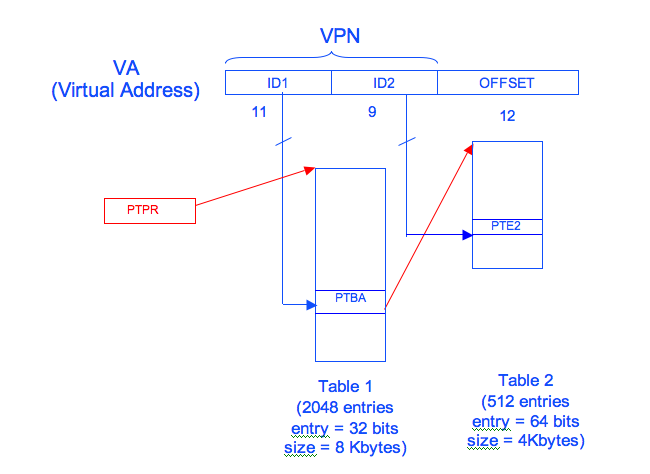
\includegraphics[scale=0.35]{include/img/pages_table_levels.png}
          \caption{La table des pages et sa
            hiérarchie~\citep{tsar2008web}.}
          \label{fig:page-table}
        \end{figure}
        \FloatBarrier
        %% TODO: barrier here ?
      \end{paragraph}
      
      \begin{paragraph}{Le noyau:}
        Lors du passage en mode noyau, la MMU est désactivée. A partir de cet
        instant, toutes les adresses manipulées par le processeur seront des
        adresses physiques. Or, celles-ci sont sur 32 bits. Pour contourner
        cette limite, ALMOS exploite deux caractéristiques \benumline \item les
        processeurs récents disposent des registres d'extension d'adresses \item
        l'architecture clusterisée de TSAR numérote ces derniers par un système
        de coordonnées $cid = (x, y) | 0 \leq x,y \leq 255$ \eenumline. On va
        donc utiliser ces $x$ et $y$, que l'on va concaténer à l'adresse
        physique sur 32 bits, pour obtenir une adresse physique sur 40 bits.
      \end{paragraph}

      
  \section{Objectifs}

    La problématique soulevée en~\ref{sec:multi-noyau} est celle à laquelle nous
    allons répondre dans le cadre de ce stage. Plus précisément, il s'agit de
    définir et de mettre en place les mécanismes suivants:
    
    \begin{itemize}
      \item assurer la création et la migration de processus mono-threads entre
        clusters
      \item ajouter le support du multi-threading
      \item ré-implémenter le composant d'ALMOS appelé DQDT (Distributed
        Quaternary Decision Tree), assurant la vision globale de l'occupation
        des ressources matérielles de la plateforme, et par conséquent
        reponsable du placement des ressources sur celle-ci.
    \end{itemize}

    \chapter{Conclusion}
\label{sec:conclusion}


  }
  {
    %% ENGLISH PART HERE
  }

  \bibliographystyle{plainnat}
  \bibliography{src/references}
  \ifr {\addcontentsline{toc}{section}{Bibliographie}}
       {\addcontentsline{toc}{section}{References}}

\end{document}
